\section{First Order Difference Equations}
    For some problems, we need to model a discrete process. Differential equations model a continuous process, while \textbf{difference equation}s model a discrete process. An example is modelling population growth of a species whose generations do not overlap. The population $y_{n+1}$ of the species in the year $n+1$ is some function of $n$ and the population $y_N$ in the preceding year:
    \begin{equation*}
        y_{n+1} = f(n, y_n) \qquad n \in \textbf{N}
    \end{equation*}
    This is a \textbf{first order difference equation} since it only depends on the step before it. The equation is \textbf{linear} if $f$ is a linear function of $y_n$; otherwise, it is \textbf{nonlinear}. A \textbf{solution} of the difference equation is a sequence of numbers $y_0, y_1, y_2, \dots$ that satisfy the equation for each $n$. There also must be an \textbf{initial condition}. 
    $$ y_0 = \alpha $$
    Now for convenience, temporarily let $f(y_n) = f(n, y_n)$.
    $$ y_1 = f(y_0) $$
    $$ y_2 = f(y_1) = f[f(y_0)] $$
    $$ y_1 = f(y_2) = f[f[f(y_0)]] = f^3(y_0) $$
    $$ y_n = f(y_{n-1}) = f^n(y_0) $$
    \indent Solutions for which $y_n$ has the same value for all $n$ are called \textbf{equilibrium solutions}. You can find this by setting $y_{n+1} = y_n$, and solve
    \begin{equation*}
        y_n = f(y_n)
    \end{equation*}
    for $y_n$.
    \newline \indent \textbf{Linear Equations}. These could be of the form
    \begin{equation*}
        y_{n+1} = \rho_n y_n \qquad n \in \textbf{N}
    \end{equation*}
    THe reproduction rate $rho_n$ may differ from year to year. This can easily be solved by iteration. We obtain
    $$ y_1 = \rho_0y_0 $$
    $$ y_2 = \rho_1y_1 = \rho_0\rho_1y_0 $$
    and, in general,
    \begin{equation*}
        y_n = (\Pi_{i=0}^{n-1}\rho_i) y_0
    \end{equation*}
    If the reproduction rate is the same for all $n$, $\rho_n = \rho$, then
    \begin{equation*}
        y_{n+1} = \rho y_n
    \end{equation*}
    \begin{equation*}
        y_n = \rho^ny_0
    \end{equation*}
    The limiting behavior can easily be determined.
    \begin{equation*}
        \lim_{n \rightarrow \infty} y_n = \begin{cases}
            0, & \text{if } |\rho| < 1; \\
            y_0, & \text{if } |\rho| = 1; \\
            \text{does not exist}, & \text{if } |\rho| > 1;
        \end{cases}
    \end{equation*}
    The equilibrium solution $y_n = 0$ is asymptotically stable for $|\rho| < 1$ and unstable for $|\rho| > 1$.
    \newline\indent
    If a population has immigration or emigration, we must have a $b_n$ as the net increase in population in year $n$ due to immigration.
    \begin{equation*}
        y_{n+1} = \rho y_n + b_n 
    \end{equation*}
    We can solve for $y_n$ through iteration as well.
    $$ y_1 = \rho y_0 + b_0 $$
    $$ y_2 = \rho(\rho y_0 + b_0) + b_1 = \rho^2y_0 + \rho b_0 + b_1 $$
    $$ y_3 = \rho(\rho^2y_0 + \rho b_0 + b_1) + b_2 = \rho^3 y_0 + \rho^2 b_0 + \rho b_1 + b_2 $$
    and in general,
    $$ y_n = \rho^n y_0 + \sum_{j = 0}^{n-1} \rho^{n-1-j} b_j $$
    The more general solution for linear equations of the form
    \begin{equation*}
        y_{n+1} = \rho_n y_n + b_n
    \end{equation*}
    then by iterations,
    \begin{equation*}
        y_n = (\Pi_{i=0}^{n-1} \rho_i) y_0 + \sum_{i=0}^{n-1} (\Pi_{j = i + 1}^{n - 1} \rho_j) b_{n-1}
    \end{equation*}
    The first term on the right side represents thr descendants of the original population.
    \newline \indent
    If $b_n = b \neq 0$,
    $$y_{n+1} = \rho y_n + b$$
    and from the previous equation the solution is
    \begin{equation*}
        y_n = \rho^ny_0 + (1 + \rho + \rho^2 + \dots + \rho^{n-1})b
    \end{equation*}
    or for $\rho \neq 1$,
    \begin{equation*}
        y_n = \rho_n y_0 + \frac{1 - \rho^n}{1 - \rho}
    \end{equation*}
    which is the same as
    \begin{equation*}
        y_n = \rho^n (y_0 - \frac{b}{1 - \rho}) + \frac{b}{1 - \rho}
    \end{equation*}
    which makes the limit behavior of $y_n$ more clear. For $\rho = 1$,
    \begin{equation*}
        y_n = y_0 + nb
    \end{equation*}
    The limit behavior is defined by 
    \begin{equation*}
        \lim_{n \rightarrow \infty} y_n = \begin{cases}
            b/(1 - \rho), & \text{if } |\rho| < 1; \\
            unbounded, & \text{if } |\rho| = 1; \\
            \text{does not exist}, & \text{if } |\rho| > 1;
        \end{cases}
    \end{equation*}
    when $|\rho|$ is not less than 1, it converges to $y_0$, if $y_0 = b/(1 - \rho)$ since this is an equilibrium solution.
    \newline \indent
    The model can also be used for interest, where $\rho_n = 1 + r_n$, where $r_n$ is the interest rate, and $b_n$ is the amount deposited or withdrawn.
    \newline \indent
    \textbf{Nonlinear Equations}. Consider the logistic difference equation
    \begin{equation*}
        y_{n + 1} = \rho y_n (1 - \frac{y_n}{k})
    \end{equation*}
    If we scale $y_n$ to $u_n = y_n/k$
    \begin{equation*}
        u_{n+1} = \rho u_n (1 - u_n)
    \end{equation*}
    ($\rho = k\rho$), a positive parameter. We can find an equilibrium solution by setting $u_{n+1} = u_n$.
    \begin{equation*}
        u_n = \rho u_n - \rho u_n^2
    \end{equation*}
    which gives us
    \begin{equation*}
        u_n = 0, \quad u_n = \frac{\rho - 1}{\rho}
    \end{equation*}
    To check if these equilibrium solutions are asymptotically stable or unstable, we can use linear approximations. Near $u_n = 0$, $u_n^2$ is small compared to $u_n$. So,
    \begin{equation*}
        u_{n+1} \approx \rho u_n
    \end{equation*}
    We already know that this only approaches 0 for $|\rho| < 1$, or $0 < \rho < 1$ since $\rho$ is positive. So $u_n = 0$ is stable for $0 < \rho < 1$.
    \newline \indent
    To test solutions in the neighborhood of $u_n = (\rho - 1) / \rho$, we write
    \begin{equation*}
        u_n = \frac{\rho - 1}{\rho} + v_n
    \end{equation*}
    where $v_n$ is small. By substituting this into $u_{n+1} = \rho u_n (1 - u_n)$, we get
    \begin{equation*}
        v_{n+1} = (2 - \rho) v_n - \rho v_n^2
    \end{equation*}
    Since $v_n$ is small, $v_n^2 \approx 0$.
    \begin{equation*}
        v_{n+1} = (2 - \rho) v_n
    \end{equation*}
    In the same manner we know $v_n \rightarrow 0$ as $n \rightarrow \infty$ for $|2 - \rho| < 1$, or $1 < \rho < 3$. Therefore, in this range of values for $\rho$, $u_n = (\rho - 1) / \rho$ is an asymptotically stable equilibrium solution. $\rho = 1$ is an \textbf{exchange of stability} from one equilibrium solution to the other.
    \newline \indent
    If $\rho > 3$, the solution will oscillate between two values; it is period 2. At about $\rho = 3.449$, the solution becomes periodic with period 4. The appearance of a new solution at a certain parameter value is called a \textbf{bifurcation}.
    \begin{center}
        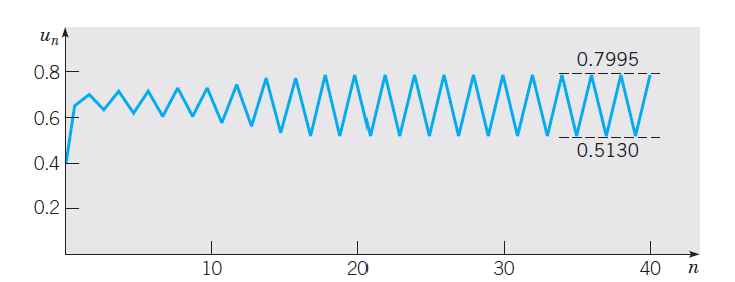
\includegraphics[width=200pt]{period.png}
    \end{center}
    \indent
    The $\rho$-values at which the successive period doublings occur approach a limit that is approximately 3.57, so for $\rho > 3.57$, the solutions have some regularity. It's fine structure is unpredictable, hence the term \textbf{chaotic}. One of the features of chaotic solutions is extreme sensitivity to initial conditions.